%-------------------------------------------------------------------------------
% Preamble
%-------------------------------------------------------------------------------

\documentclass{article}


%Packages
\usepackage{
	siunitx, % units
  	graphicx, % for images
	natbib,
	booktabs,
	rotating, % rotate figure
}
\usepackage[letterpaper]{geometry}
\renewcommand{\thefigure}{S\arabic{figure}}
\renewcommand{\thetable}{S\arabic{table}}
\newcommand{\round}[1]{\num[round-mode=places,round-precision=3]{#1}}
\usepackage[breaklinks=true,hidelinks]{hyperref}
\graphicspath{{../../figs/}{./}}

%-------------------------------------------------------------------------------
% Title and Authors
%-------------------------------------------------------------------------------

\title{Supplemental Information for\\``Heavy rainfall in Paraguay during the 2015-2016 austral summer: causes and subseasonal-to-seasonal predictive skill''}
\author{James Doss-Gollin\and \'{A}ngel G. Mu\~{n}oz  \and Simon J. Mason \and Max Past\'{e}n }
\date{\today}

\begin{document}

%% Necessary!
\maketitle

This document contains several supplemental figures referenced in the main text.
Further supporting information is available in the form of source code at \url{github.com/jdossgollin/PYFloods}.

\listoftables
\listoffigures

\clearpage

\begin{table}
	\centering
	\begin{tabular}{lrr}
		\toprule
		{} &  NDJF 2015-16 &  Climatology \\
		WT &               &              \\
		\midrule
		1     &         0.273 &        0.213 \\
		2     &         0.231 &        0.185 \\
		3     &         0.107 &        0.156 \\
		4     &         0.207 &        0.156 \\
		5     &         0.132 &        0.150 \\
		6     &         0.050 &        0.140 \\
		\bottomrule
	\end{tabular}
	\caption{Weather type (WT) occurrence fraction during NDJF 2015-16 and Climatology}
\end{table}

\begin{table}
	\centering
	\begin{tabular}{lrrrr}
		\toprule
		{} &  EOF 1 &  EOF 2 &  EOF 3 &  EOF 4 \\
		WT &        &        &        &        \\
		\midrule
		1  & -0.325 &  1.035 & -1.015 &  0.124 \\
		2  & -0.887 &  0.519 &  0.647 & -0.812 \\
		3  &  1.312 &  0.325 &  0.208 &  0.075 \\
		4  &  0.190 & -0.807 & -0.120 & -0.844 \\
		5  & -0.307 & -0.849 & -0.741 &  0.826 \\
		6  & -0.334 &  0.057 &  1.093 &  1.033 \\
		\bottomrule
		\end{tabular}
	\caption{
		Centroids of each weather type in 4-dimensional phase space, where each dimension is an EOF of \SI{850}{\hecto\pascal} streamfunction over the weather typing region. 
		These centroids are chosen by choosing the $K$-means partition which maximizes the Classifiability Index; see Methods.
		The weather type for each day is computed by projecting the \SI{850}{\hecto\pascal} onto its leading four EOFs, re-scaling the EOFs as discussed in Methods, and identifying the nearest (Euclidean distance) centroid.
	}
\end{table}

\clearpage

\begin{figure}
	\centering
  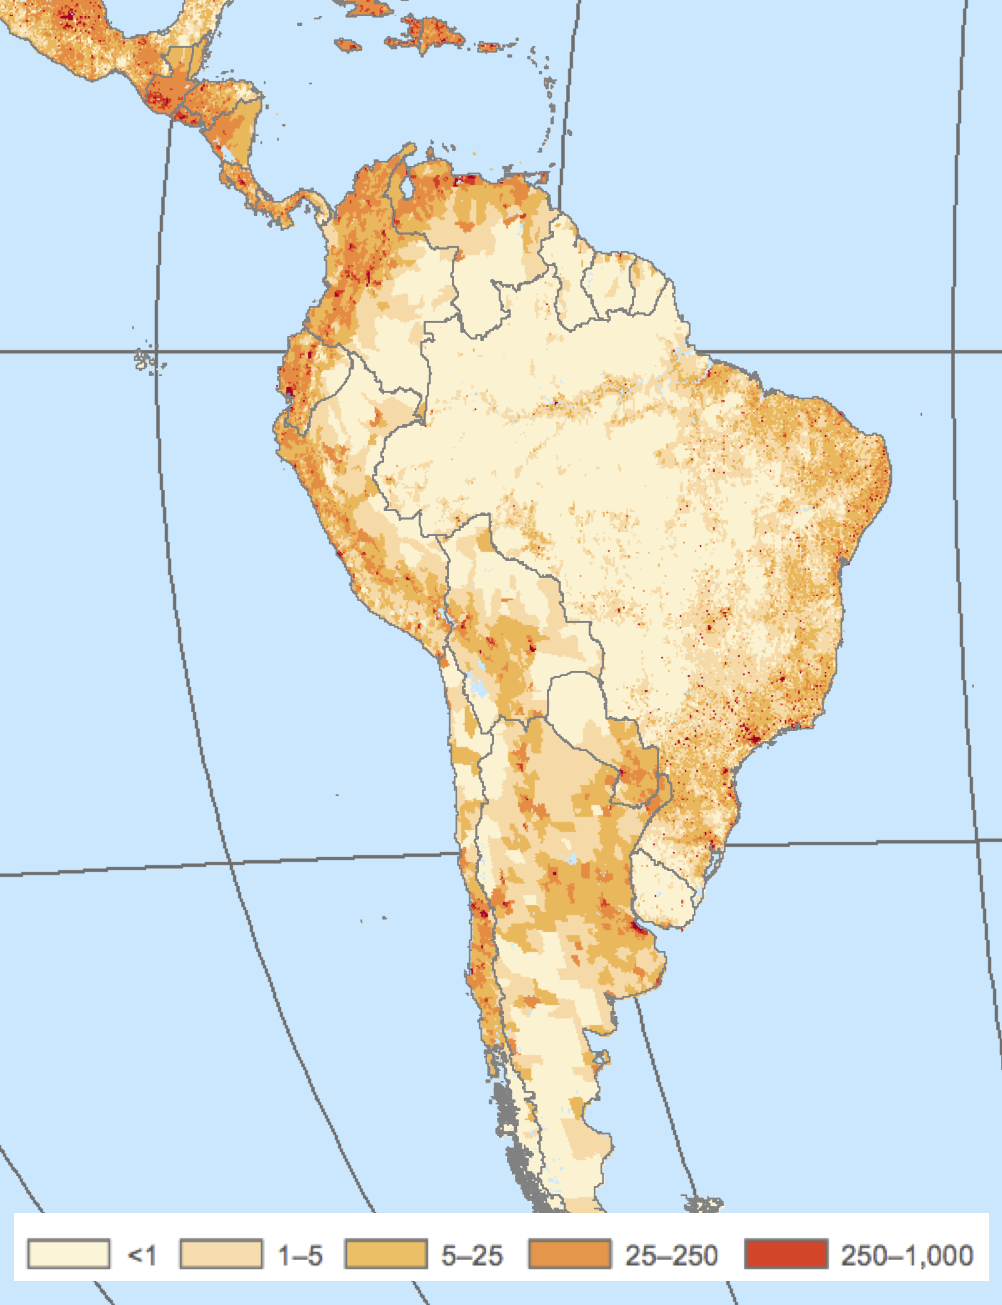
\includegraphics[width=\textwidth,height=0.6\textheight,keepaspectratio=true]{gpw-v4-2015.png}
	\caption{
		Gridded estimate of population density (color; in units of persons per square kilometer) from \citet{GPWv4}.
	}
\end{figure}

\begin{figure}
	\includegraphics[width=\textwidth]{mjo_ts.pdf}
	\caption{
		Evolution of the MJO during NDJF 2015-16.
		Points are plotted on RMM1 ($x$-axis) and RMM2 ($y$-axis), derived from leading EOFs of OLR fields \citep{Wheeler2004}.
		Gray lines divide the plot into the eight phases used in the text.
		Colors show the time evolution of the system from 01 November 2015 (blue) to 29 February 2016 (yellow).
		Gray circle indicates the area of neutral MJO activity with amplitude $<0$.
	}
\end{figure}

\begin{figure}
	\includegraphics[width=\textwidth]{nino_34_ts.pdf}
	\caption{
		Monthly NINO 3.4 time series during the study period.
		Each month from November 2015 through February 2016 is specifically marked with a blue dot.
		Data from \citet{Kaplan1998}.
	}
\end{figure}

\begin{sidewaysfigure}
	\includegraphics[width=\textwidth, height=\textheight, keepaspectratio=true]{nino_sst_anomalies.pdf}
	\caption{
		Monthly SST anomalies during December of three major El Ni\~{n}o events.
		Months shown are NDJF of (a,d,g,j): 1982-83, (b,e,h,k): 1997-98, and (c,f,i,l): 2015-16.
		Units are in \si{\celsius}.
		SST data from \citet{Reynolds2002}.
		Also shown are rainfall anomalies over South America, from \citet{Chen2008}.
		Rainfall contour intervals are \SI{1}{\milli\meter\per\day}.
	}
\end{sidewaysfigure}

\begin{figure}
	\noindent\includegraphics[width=6.4in]{sst_anomalies.pdf}
	\caption{
		Pearson correlation, at monthly time step, of  sea surface temperature (SST) anomalies \citep{Reynolds2002} with four leading EOFs of \SI{850}{\hecto\pascal} streamfunction over the weather typing region, shown with a black box.
		Central Southern Atlantic Dipole is shown with a blue box.
		(a): EOF 1; (b): EOF2; (c): EOF3; (d): EOF4.
	}\label{fig:sst-anomalies}
\end{figure}


\begin{figure}
	\includegraphics[width=\textwidth]{wt_classifiability.pdf}
	\caption{
		Classifiability index (see Methods) calculated for several chosen values of $K$, representing the number of weather types produced.
		Results are produced with only 75 simulations for each $K$.
	}
\end{figure}

\clearpage
\bibliographystyle{ametsoc2014}
\bibliography{../library}

\end{document}
